% Chapter Template

\chapter{Introducción} % Main chapter title

\label{Chapter1} % Change X to a consecutive number; for referencing this chapter elsewhere, use \ref{ChapterX}

%----------------------------------------------------------------------------------------
%	SECTION 1
%----------------------------------------------------------------------------------------

\section{Seguridad en Internet}

Es posible encontrar múltiples definiciones de lo que se entiende por seguridad en la red o Internet. Por ejemplo, Stallings se refiere a ello como la protección que se proporciona a un sistema de la información para preservar la integridad, disponibilidad y confidencialidad de sus recursos, tanto software como hardware \cite{Stallings2016}. Por otro lado, la empresa Cisco la define como la actividad destinada a proteger la usabilidad y la integridad de la red y datos. Al igual que la anterior, engloba medios software y hardware \cite{cisco}. Estas son tan solo dos ejemplos de las muchas acepciones que existen, pero es posible observar que coinciden en gran medida en los aspectos que la seguridad, en términos de Internet, debería garantizar. Ambas también establecen los mismos objetivos a proteger: medios hardware y software. Es importante entender en que consisten la integridad, la disponibilidad y la confidencialidad, conjunto conocido como \textit{CIA} (\textit{Confidenciality, Integrity and Availability}). La confidencialidad asegura que datos de carácter privado no sean accedidos por personas no autorizadas; la disponibilidad permite que datos o cualquier otro tipo de recurso pueda ser utilizado sin ningún tipo de impedimento y, finalmente, la integridad preserva el contenido de los datos o comportamiento de un sistema, de manera que estos no sean modificados por alguien desautorizado. Todos estos términos pueden aplicarse a un sistema aislado, pero cuando este sistema pasa a estar en una red de millones de nodos, las amenazas se múltiplican.  

%-----------------------------------
%	SUBSECTION 1
%-----------------------------------
\subsection{Tipos de atacantes}
Se distinguen distintos tipos de atacantes: hackers, criminales y empleados. Los hackers suelen realizar ataques buscando la emoción de conseguir acceder a un sistema restringido y el reconocimiento del resto de la comunidad hacker. Son frecuentes los ataques de oportunidad que aprovechan alguna vulnerabilidad para acceder a información que luego comparten en la red. Los segundos atacantes, los criminales, constituyen bandas de hackers que se asocian para llevar a cabo ataques con fines lucrativos, generalmente contra servicios de comercio electrónico. Tratan de hacerse con datos bancarios y tarjetas de crédito que después utilizan a expensas de la víctima o venden en la red.
Estos grupos, que se han expandido por toda la red, suponen una amenaza común para todos los sistemas basados en Internet, buscan objetivos concretos y, en ocasiones, son contratados por gobiernos u otras organizaciones. Por úlimo, los empleados son individuos que ya se encuentran dentro del sistema y conocen su estructura. Sus ataques pueden estar motivados por venganza contra la organización en la que trabajan o sencillamente, por un sentimiento de derecho. Resultan, por lo tanto, los ataques más difíciles de detectar y prevenir, y solamente políticas de acceso y monitorización dentro de la organización ayudan a evitarlos\cite{Stallings2016}.

%-----------------------------------
%	SUBSECTION 2
%-----------------------------------
\subsection{Ataques de seguridad y sus motivaciones}
Las normas \textit{X.800} y \textit {RFC 4949} clasifican los ataques en dos categorías: pasivos y activos. Los ataques pasivos serían aquellos que extraen información de un sistema, pero no alteran en modo alguno a sus recursos. Un ejemplo sería la monitorización de las transmisiones realizadas entre dos sistemas, accediendo a esta información. Por otro lado, los ataques activos sí que afectan los a los recursos de un sistema e incluso a su funcionamiento. Dentro de este tipo de ataques se encuentran la suplantación, cuando un individuo u organización finge ser otra distinta; reenvio de información capturada previamente sin autorización; modificación de mensajes o la denegación de servicio, que impide el acceso normal a un servicio\cite{Stallings2016}.
En lo que respecta a las motivaciones, la gran mayoría de ataques están conducidos por el espionaje o un interés financiero. Otras motivaciones serían la diversión, el resentimiento o la ideología. No obstante, hay que tener en cuanto que muchos casos de extorsión no son reportados y confirmados, por lo que las cifras recogidas en las estadísticas no reflejan la totalidad de los ataques. Aún así, es posible contar con una referencia de los fines que persiguen algunos conocidos ataques\cite{DBIR2017}: 
\begin{itemize}
	\item Financieros: uso de credenciales robadas, uso de backdoor, spyware, phising, malware para exportar data, c2.
	\item Espionaje: phising, c2, uso de backdoor.
	\item Resto: abuso de privilegios
\end{itemize}


\section{Algunas cifras concretas}
En relación a lo anterior, existen multitud de estudios e informe que tratan de recabar información acerca del estado de la seguridad en Internet partiendo de diversas fuentes, como encuestas o ataques sufridos. Pese a que gran parte de estos estudios están realizados por empresas privadas, resultan útiles para obtener una perspectiva global del problema que supone la seguridad en Internet.


\subsection{DBIR 2017}
El DBIR (\textit{Data Breach Investigations Report}), un informe realizado por Verizon en el que participan 65 organizaciones, analiza el estado de la ciberseguridad.Según este informe hubo 1616 ataques durante el año 2016, de los que 828 supusieron la revelación de datos confidenciales. Este informe también proporciona los tipos de ataques más conocidos, así como los actores que los perpetran y sus motivaciones. Plasmando en cifras lo referido en la anterior sección, el 66\% de los ataques tenían una motivación financiera y el 33\% de espionaje. Menos del 1\% de los ataques fueron motivados por ideología o diversión. Además, el 99\% de estos ataques los llevaron a cabo individuos u organizaciones externas. Otro dato interesantes que recoge el informe es que la táctica más empleada es la de phising y que la mayoría de estos ataques van seguidos por la instación de algún tipo de malware. Finalmente, cabe mencionar que el 81\% de las brechas de seguridad se produjeron debido a credenciales inseguras o robadas. Este informe además analizar las estadísticas de los ataques reportados, proporciona algunos consejos en base a los resultados para tratar de evitarlos. Destaca, sobretodo, la necesidad de concienciar y educar acerca de las amenzadas y riesgos que existen. También pone el foco en la importancia que supone la detección temprana de un ataque y la localización de la fuente del ataque\cite{DBIR2017}. En definitiva, se trata tan solo de un informe, pero pone de manifiesto la magnitud del problema que representa la seguridad en internet.
\begin{figure}[!b]
\centering
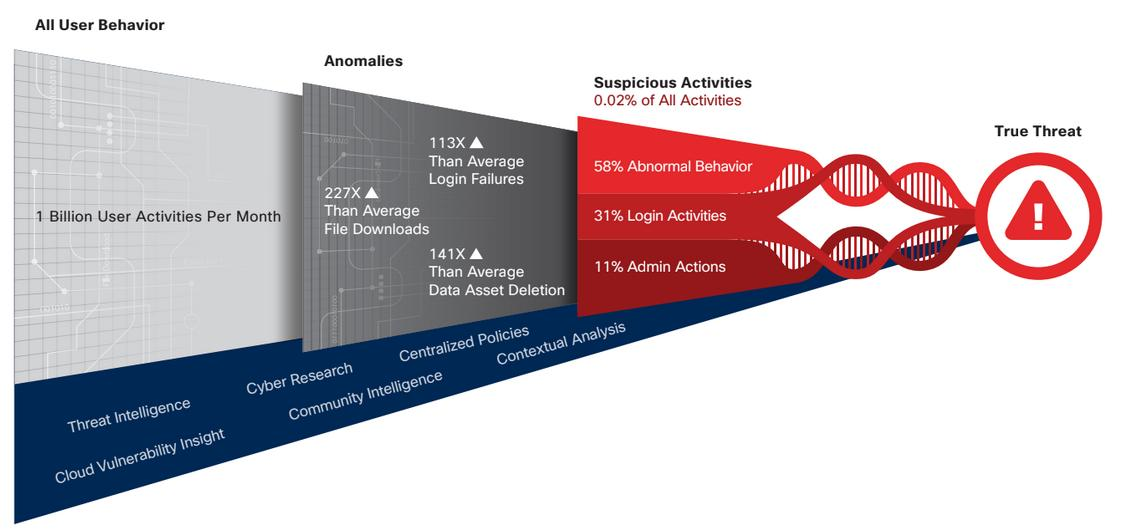
\includegraphics[width=1\textwidth]{images/userBehavior.png}
\caption{Identificación de patrones de comportamiento de usario normal}
\label{fig:behavior}
\end{figure}

\subsection{Cisco 2017 Annual Cybersecurity Report}
El grupo de investigación de seguridad de Cisco publica cada año este informe, para ayudar a las organizaciones a hacer frente a las amenazas y riesgos que surgen constantemente en la red. Entre los datos recogidos por el informe cabe destacar las razones que impiden la adopción de sistemas u otras medidas de seguridad en muchas empresas. El 35\% carecía de presupuesto, para el 28\% presentaba problemas de compatibilidad, el 25\% por la certificación y el 25 \% restante por falta de talento. Por este motivo, apenas la mitad de las alertas de seguridad que se reciben son investigadas. Cabe mencionar también el hecho de que aquellas organizaciones que aún no han sufrido ninguna brecha de seguridad están convencidas de que su red es segura, aunque esta seguridad parece cuestionable si se tiene en cuenta el grado de afectación que supone para cualquier empresa que su sistema se vea comprometido. Casi un cuarto de las empresas perdieron alguna oportunidad de negocio al sufrir un ataque y 1 de cada 5 perdió clientes. Este estudio también muestra que muchas de las empresas recurren a las soluciones de seguridad de varias empresas especializadas, por lo general más de 5, con varios productos distintos también. Todo ello supone una complejidad extra que dificulta la automatización de tareas, algo fundamental a la hora de mejorar la seguridad de un sistema. Por ejemplo, distinguir un comportamiento anómalo y sospechoso del que, según los patrones, resulta normal requiere un proceso de varias etapas que solo puede lograrse con automatización\ref{fig:behavior}.\\
En lo que se refiere a los ataques, los datos revelan que en la mayoría de ellos se distinguen las siguientes fases:
\begin{itemize}
	\item Reconomiento: los atacantes investigan, identifican y seleccionan a sus víctimas.
	\item Armamento: generación de paquetes con malware que permite el acceso remoto aprovechando una vulnerabilidad.
	\item Distribución: la carga anterior se hace llegar mediante correo, ficheros adjuntos, etc.
	\item Instalación: en el objetivo, el malware genera una puerta trasera que permite el acceso permanente de los atacantes.
\end{itemize}
Frente a los ataque, una de las medidas que propone cisco para conocer el progreso de las medidas de seguridad es el TTD (\textit{Time To Detec}. Lo define como el intervalo de tiempo que transcurre desde que un sistema se ve comprometido hasta que la amenaza es detectada. Las amenazas y ataques evolucionan muy rápidamente y en ocasiones resulta difícil identificar un ataque, aunque este sea conocido en la comunidad. De la misma manera que los sistemas de seguridad trabajan en mejorar el TTD, los atacantes desarrollan nuevas técnicas y estrategias para evitar ser detectados y disponer así de más tiempo  para perpetrar su ataque. Esta mejora en los ataques se puede medir con el TTE (\textit{Time To Evolve}, el tiempo que tarda un atacante en modificar el modo en que cierto malware es distribuido o en cambiar de táctica.  


